\documentclass{article}

\usepackage{amsmath, amsthm, amssymb}
\usepackage{graphicx, dsfont}

\title{Notes for MATH 3210: Foundation of Analysis I}
\author{Jing Guo}
\date{\today}

\newtheorem*{theorem}{Theorem}
\newtheorem*{remark}{Remark}

\newcommand{\abs}[1]{\left| #1 \right|}
\newcommand{\inpro}[2]{(#1 \mid #2)}
\newcommand{\norm}[1]{\| #1 \|}

\begin{document}

    \maketitle
    \tableofcontents
    
    \section{Ring and Field}
    
    Notations:
    
    \begin{itemize}
        \item $\mathbb{N}$: The set of natural numbers;
        \item $\mathbb{Z}$: The set of integers (ring, not field, has no inverse);
        \item $\mathbb{Q}$: The set of rational numbers;
        \item $\mathbb{R}$: The set of real numbers (ring and field).
    \end{itemize}
    
    \subsection{Ring}
    
    The set $A$ has two binary operations, addition and multiplication.
    
    For any $a, b \in A$,
    
    \begin{align*}
        A \ast A &\to A \\
        a, b &\to a + b
    \end{align*}
    
    \subsubsection{Addition Axiom}

    \begin{enumerate}
        \item $a + b = b + a$ (commutative)
        \item $(a + b) + c = a + (b + c)$ (associative)
        \item There is an element $0$ such that $a + 0 = a$ (additive identity)
        \item There exists $-a$ (additive inverse) such that $a + (-a) = 0$
    \end{enumerate}

    \subsubsection{Multiplication Axiom}
    
    \begin{enumerate}
        \item $a \cdot b = b \cdot a$
        \item $(a \cdot b) \cdot c = a \cdot (b \cdot c)$
        \item There is an element $1$ such that $a \cdot 1 = a$ and $0 \neq 1$
        \item $a \cdot (b + c) = a \cdot b + a \cdot c$ (distributive)
    \end{enumerate}

    \subsection{Field}
    
    $A$ is a field if $A$ is a \textit{ring} for any $a \in A$ and $a \neq 0$, there exists $a^{-1}$ (inverse of $a$) such that $a \cdot a^{-1} = 1$.
    
    $A$ has no zero divisors if $x \neq 0, y \neq 0 \rightarrow x \cdot y \neq 0$
    
    \textbf{Example}: $x, y \in A$, $x \neq 0$, $y \neq 0$, $xy = 0$
    
    \begin{displaymath}
    \begin{bmatrix}
        1 & 0 \\
        0 & 0
    \end{bmatrix}
    \cdot
    \begin{bmatrix}
        0 & 0 \\
        0 & 1
    \end{bmatrix}
    =
    \begin{bmatrix}
        0 & 0 \\
        0 & 0
    \end{bmatrix}
    \end{displaymath}
    
    \subsection{Construction of Integers}
    
    We need to construct $\mathbb{Z}$ from $\mathbb{N}$ with \textbf{localization}.
    
    \begin{displaymath}
        \mathbb{N} = \{ 0, 1, 2, 3, \ldots \}
    \end{displaymath}
    
    Set of equivalence class: $\mathbb{N} \times \mathbb{N} / \sim$
    
    Equivalence relation: $(a, b) \sim (a', b')$ if $a + b' = b + a'$, since $a - b = a' - b'$
    
    \begin{gather*}
        (a, b) \sim (a', b') \sim (a'', b'') \\
        a' + b'' = b' + a'' \\
        \boldsymbol{(a + b'') + b'} = (a + b') + b''
        = b + a' + b'' = b + b' + a'' = \boldsymbol{(a'' + b) + b'} \\
        \therefore a + b'' = a'' + b \\
        \therefore (a, b) \sim (a'', b'')
    \end{gather*}
    
    We then should define addition:
    
    \begin{equation} \label{eq:add1}
        [(a, b)] + [(a', b')] = [(a + a', b + b')]
    \end{equation}
    
    \begin{equation} \label{eq:add2}
        [(a_{1}, b_{1})] + [(a', b')] = [(a_{1} + a', b_{1} + b')]
    \end{equation}
    
    Equation \ref{eq:add1} and equation \ref{eq:add2} are equal since independent of choice of equivalence classes:
    
    \begin{gather*}
        a + a' + b_{1} + b' = a_{1} + a' + b + b' \\
        a + b_{1} = a_{1} + b
    \end{gather*}
    
    Additive identity: $0 = [(0, 0)]$
    
    For example: $[(a, b)] + [(b, a)] = [(a + b, a + b)] = [(0, 0)] = 0$
    
    We then need to define multiplication:
    
    \begin{displaymath}
        [(a, b)] \cdot [(a', b')] = [(aa' + bb', ab' + a'b)]
    \end{displaymath}
    
    \begin{align*}
        &(a - b)(a' - b') \\
     = \quad &aa' - ab' - a'b + bb' \\
     = \quad &(aa' + bb') - (ab' + a'b)
    \end{align*}
    
    Multiplicative identity: $1 = [(1, 0)]$
    
    For example: $[(a, b)] \cdot [(1, 0)] = [(a, b)]$
    
    $\therefore \mathbb{N} \times \mathbb{N} / \sim$ is a ring, that is, $\mathbb{Z}$.
    
    \begin{align*}
        \mathbb{N} &\longrightarrow \mathbb{Z} \\
        m &\longrightarrow [(m, 0)] \\
        -m &\longrightarrow [(0, m)] = -[(m, 0)]
    \end{align*}
    
    For example:
    
    \begin{align*}
        [(a, b)] &= [(a, 0)] + [(0, b)] \\
                   &= [(a, 0)] - [(b, 0)]
    \end{align*}
    
    \subsection{Construction of Fractions (Rational Numbers)}
    
    We need to show that $K$ is a field (with addition and multiplication). Assume $A$ is a commutative ring with no zero divisors, and $A^{\ast} = A - \{ 0 \}$.
    
    $A \times A^{\ast} = \{ (a, b) \mid a, b \in A, b \neq 0 \}$
    
    Set of equivalence classes: $K = (A \times A^{\ast}) / \sim$ (elements of $K$ are fractions)
    
    We first need to define addition:
    
    \begin{align*}
        (a, b) &\sim (a', b') \\
        \frac{a}{b} &= \frac{a'}{b'} \\
        ab' &= a'b
    \end{align*}
    
    $[(a, b)]$: The equivalence class of $(a, b)$
    
    \begin{align*}
        [(a, b)] + [(a', b')] &= [(ab' + a'b, bb')] = \frac{ab' + a'b}{bb'} \\
        [(0, 1)] &= 0 \in K \quad \text{(additive identity)} \\
    \end{align*}
    
    The following is to prove that it is independent of the choice of equivalence class:
    
    \begin{align*}
        [(a_{1}, b_{1})] + [(a', b')] &= [(a_{1}b' + a'b_{1}, b_{1}b')] \\
        \therefore (ab' + a'b) \cdot b_{1}b' &= (a_{1}b' + a'b_{1}) \cdot bb' \\
        \therefore left &= right
    \end{align*}
    
    We then need to define multiplication:
    
    \begin{align*}
        [(a, b)] [(a', b')] &= [(aa', bb')] = \frac{aa'}{bb'} \\
        [(1, 1)] &= 1 \in K \quad \text{(multiplicative identity)}
    \end{align*}
    
    \textbf{Examples}:
    
    \begin{align*}
        [(x, y)] + [(0, 1)] = [(x, y)] \\
        [(x, y)] \cdot [(1, 1)] = [(x, y)] \\
        [(x, y)] \neq [(0, 1)]
    \end{align*}
    
    So we need to show that $K$ is a field:
    
    \begin{align*}
        [(x, y)] \cdot [(y, x)] &= [(xy, xy)] = [(1, 1)] \quad \text{(Non-zeros have inverse)} \\
        \because &ab' = a'b \\
                       &(a, b) \sim (a', b') \\
        \therefore &[(xy, xy)] = [(1, 1)]
    \end{align*}
    
    \textbf{Therefore} $K$ is a field of fractions of $A$.
    
    We need to show the following map is injective:
    
    If $A = \mathbb{Z}$ and $K = \mathbb{Q}$:
    
    \begin{align*}
        A &\longrightarrow K \quad \text{{(injective)}} \\
        x &\longrightarrow [(x, 1)] \\
        x + y &\longrightarrow [(x + y, 1)] = [(x, 1)] + [(y, 1)] \\
        x \cdot y &\longrightarrow [(xy, 1)] = [(x, 1)] \cdot [(y, 1)] \\
        \text{Comm. ring without } 0 &\longrightarrow \text{Field containing the ring}
    \end{align*}

    Assume $[(a, 1) = [(b, 1)]]$ where $a, b \in A$:
    
    \begin{align*}
        &a \cdot 1 = b \cdot 1 \Rightarrow a = b \\
        &\therefore \text{The map is injective.}
    \end{align*}
    
    $P(x) = a_{0}x^{n} + a_{1}x^{n - 1} + a_{2}x^{n - 2} + \cdots + a_{n}, a \in R$
    
    Ring of polynomials: $P(x) \times Q(x) \Rightarrow R(x)$ (with no zero divisors)
    
    \subsection{Ordered Set}
    
    \subsubsection{Partial Order}
    
    $(S, \leq)$ is a (partially) ordered set (poset), $\forall x, y, z \in S$:
    
    \begin{enumerate}
        \item $x \leq$ x
        \item $x \leq y, y \leq x \Rightarrow x = y$
        \item $x \leq y, y \leq z \Rightarrow x \leq z$
    \end{enumerate}

    \subsubsection{Total Order}

    Total/Linear order: Either $x \leq y$ or $y \leq x$.
    
    Ordered field is a field $K$ with $\leq$ total order.
    
    \textbf{Definition}:
    
    \begin{enumerate}
        \item If $x \leq y$ then $x + z \leq y + z$ and
        \item if $x \geq 0, y \geq 0$ then $x \times y \geq 0$
    \end{enumerate}

    There is no total order in complex numbers.

    \textbf{First example}:
    
    \begin{gather*}
        \mathbb{Q} = \{ (a, b) \}, (a, b) = \frac{a}{b} \\
        \text{Since} \quad a \geq 0, b > 0
    \end{gather*}
    
    $\therefore \mathbb{Q}$ is an ordered set.
    
    \textbf{Second example}:
    
    \begin{align*}
        x \geq 0 &\Leftrightarrow -x \leq 0 \\
        x \geq 0 &\Rightarrow x^{2} \geq 0 \\
        x \leq 0 &\Rightarrow (-x)^{2} = x^{2} \geq 0
    \end{align*}
    
    \begin{align*}
        1^{2} = 1 > 0 \\
        2 > 1 \\
        3 > 2 \\
        \vdots \\
        n > n - 1
    \end{align*}
    
    \subsubsection{Least-upper-bound Property}
    
    $\mathbb{Q}$: Ordered field of rational numbers (with gaps)
    
    Least-upper-bound property: $K$ has least-upper-bound property if any bounded subset $E \subset K$ has least upper bound.
    
    $K$ is a field with order relation $\leq$, $E \subset K$ and $E$ is \textit{bounded above} if $\exists \alpha \in K$ such that $p \leq \alpha, p \in E$.
    
    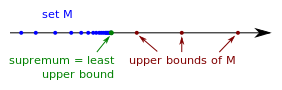
\includegraphics{supremum}
    
    $\beta$ is the \textit{least-upper-bound} of $E$ if
    
    \begin{enumerate}
        \item $\beta$ is an upper bound,
        \item for any other upper bound $\alpha$, we have $\beta \leq \alpha$.
    \end{enumerate}

    We call $\beta = \sup E$.
    
    We then need to prove that $\mathbb{Q}$ does not have least-upper-bound property, that is, there are gaps in $\mathbb{Q}$.
    
    \begin{proof}
        \begin{align*}
            E = \{ q \in \mathbb{Q} : q^{2} \leq 2 \} \quad &\Rightarrow \quad  \text{no } \sup E \\
            q \in E \Leftrightarrow - q \in E \quad &\text{and} \quad q \geq 0 \\
        \end{align*}
            
        Let $p \in \mathbb{Q}$ such that $p \geq 0, p^{2} > 2$.
            
        \begin{align*}
            \therefore &p^{2} > 2 \geq q^{2} \Rightarrow p^{2} \geq q^{2} \\
                            &p^{2} - q^{2} = (p + q)(p - q) \geq 0 \quad \text{(property of ordered field)} \\
            \because  &p \geq 0, q > 0 \\
            \therefore &p + q \geq 0 + q = q \geq 0 \\
            \therefore &p \geq q \\
                            &p \in \mathbb{Q}, p \geq 0, p^{2} > 2 \text{ are upper bound of } E.
        \end{align*}

        Remark: Let $p$ be upper bound of $E$, $\forall q \in E, q \leq p, p > 0$.
        
        Define $p'$:
        
        \begin{displaymath}
            p' = p - \frac{p^{2} - 2}{p + 2} = \frac{2p + 2}{p + 2} = 2\frac{p + 1}{p + 2}
        \end{displaymath}
        
        \begin{displaymath}
            \therefore p'^{2} - 2 = 2\frac{p^{2} - 2}{(p + 2)^{2}}
        \end{displaymath}
        
        In the above equation, $p^{2} - 2 \leq 0$ and $(p + 2)^{2} \geq 0$.
        
        Assume $p \in E \Rightarrow p^{2} \leq 2 \Rightarrow p^{2} - 2 \leq 0$.
        
        $\therefore p'^{2} - 2 \leq 0 \Rightarrow p' \in E \text{ and } p' \geq p$.
        
        $\therefore \text{Either } p' = p \text{ or } p' > p$.
        
        But neither of them is possible since $\sqrt{2}$ is irrational:
        
        \begin{align*}
            &p = p' \Rightarrow p^{2} = 0, p \in \mathbb{Q} \text{ but } p \text{ is irrational.} \\
            &\therefore p \notin E. \text{ All upper bounds of } E \text{ are } \{ p \in \mathbb{Q}, p^{2} > 2 \}
        \end{align*}
        
        $r$: an upper bound, and $r^{2} \geq 2$
        
        \begin{alignat*}{2}
            r' &= r - \frac{r^{2} - 2}{r^{2} + 2} \quad &&\therefore r' < r \\
            r'^{2} - 2 &= 2\frac{r^{2}}{(r + 2)^{2}} > 0 \quad &&\therefore r'^{2} > 2
        \end{alignat*}
        
        $\therefore r'$ is an upper bound of $E$.
        
        So we have no upper bound property in $E$.
    \end{proof}
    
    \subsection{Real Numbers}
    
    \subsubsection{Construction of Real Numbers}

    \begin{theorem}
        There exists a total ordered field $\mathbb{R}$ which has least upper bound property. So every subset $E \subset \mathbb{R}$, are bounded above, has a supremum.
        
        Such field is \textbf{unique}.
    \end{theorem}

    \begin{align*}
        K &\xrightarrow{\varphi} K' \\
        \varphi(x + y) &= \varphi(x) + \varphi(y) \\
        \varphi(x \cdot y) &= \varphi(x) \cdot \varphi(y) \\
        \text{if bijective, then isomorphism;} &\text{ otherwise, morphism.}
    \end{align*}
    
    History of construction of real numbers: Dedekind used cuts and Cantor used Cauchy sequence, which works for more general occasions, in 1872.
    
    What is \textit{cuts}?
    
    \begin{align*}
        &E \subset \mathbb{Q}, E \neq \mathbb{Q} \rightarrow E \text{ is bounded above} \\
        &q \in \mathbb{Q}, E_{q} = \{ p \in \mathbb{Q} : p < q \} \\
        &\text{If } \alpha \in E, \beta < \alpha \Rightarrow \beta \in \alpha \\
        &\gamma \in E, \delta \in E, \delta > \gamma
    \end{align*}
    
    \subsubsection{Archimedean Property}
    
    \begin{theorem}[Archimedean Property]
        \begin{align*}
            x, y \in \mathbb{R}&, x > 0, y > 0 \\
            \exists n \in \mathbb{Z}_{+}&, n \cdot x > y
        \end{align*}
    \end{theorem}

    \begin{proof}
        Assume $\{ nx \mid n \in \mathbb{Z} \}$ is bounded above, i.e. has least upper bound property.
        
        \begin{align*}
            &\exists \alpha = \sup \{ nx \mid n \in \mathbb{Z} \} \\
            &n \cdot x \leq \alpha, \forall n \text{ and } \alpha - x < \alpha \\
            \because \quad &\alpha = \sup \{ nx \mid n \in \mathbb{Z} \} \\
            \therefore \quad &\alpha - x \text{ is NOT an upper bound.} \\
            &\exists m \text{ such that } \alpha - x < n \cdot x \\
            \therefore \quad & \alpha < (n + 1) x \\
            \therefore \quad & \text{Contridication.} \\
            \therefore \quad &\{ nx \mid n \in \mathbb{R} \} \text{ is not bounded above.} \\
        \end{align*}
    \end{proof}

    \subsubsection{Density of Real Numbers}
    
    \begin{proof}
        Assume $x, y \in \mathbb{R}$ and $x < y$.
        
        There exists $q \in \mathbb{Q}$ such that $x < q < y$. Because $y - x > 0$ and $1 > 0$, so there exists $n$ such that $n(y - x) > 1$.
        
        \begin{align*}
            nx < m_{1}, \quad & m_{1} \in \mathbb{Z} \\
            -nx < m_{2}, \quad & m_{2} \in \mathbb{Z} \\
            \therefore -m_{2} < &nx < m_{1}
        \end{align*}
        
        Conclusion: $\exists m \in \mathbb{Z}, m - 1 \leq nx < m$, so $nx < m \leq nx + 1 < ny$.
        
        \begin{align*}
            nx < m < ny \\
            m \leq mx + 1 \\
            \therefore x < \frac{m}{n} < y
        \end{align*}
    \end{proof}

    \subsubsection{Property of Real Numbers}
    
    We have $x > 0, y > 0, n \geq 2$, and $y^{n} = x$, such $y$ is unique.
    
    We first need to prove \textbf{uniqueness}:
    
    \begin{proof}
    We have $y_{1}, y_{2} > 0, y_{1}^{n} = x, y_{2}^{n} = x \Rightarrow y_{1} = y_{2}$
    
    We assume $y_{1} \neq y_{2}$ and $0 < y_{1} < y_{2}$. If $a > 0$, then $ay_{1} > ay_{2}$.
    
    We claim $y_{1}^{n} < y_{2}^{n}$, then we apply mathematical induction:
    
    When $n = 1$, $y_{1} < y_{2}$.
    
    \begin{align*}
        y_{1}y_{1}^{n} &< y_{1}^{n}y_{2} < y_{2}y_{2}^{n} \\
        y_{1}^{n + 1} &< y_{2}^{n + 1} \\
        \therefore y_{1}^{n} &< y_{2}^{n} \\
    \end{align*}
    
    But they should both be equal to $x$, therefore we have a contradiction.
    \end{proof}
    
    We then need to prove \textbf{existence}:
    
    \begin{displaymath}
        E = \{ t \in \mathbb{R} \mid t^{n} < x, x > 0, x \in \mathbb{R} \}
    \end{displaymath}
    
    \begin{proof}
        We first need to show that set $E$ is not empty.
        
        We construct $t = \frac{x}{x + 1} \Rightarrow 0 < t < 1$ and $t^{n} < t^{n - 1} < \cdots < t < 1$
        
        \begin{align*}
            t = \frac{x}{x + 1} \\
            x = t + tx \\
            t = x - tx < x \\
            \therefore t^{n} < t < x \\
        \end{align*}
    \end{proof}
    
    We then need to show that $E$ is bounded above:
    
    \begin{proof}
        Suppose $S \geq x + 1 \Rightarrow S > 1$, so $S^{m} > S^{m - 1} > \cdots > S$, therefore $S^{m} > x + 1 > S$.
        
        It follows that if $t \in E$, then $t < x + 1 \Rightarrow x + 1$ is an upper bound of $E$.
        
        $\exists y = \sup E, y > 0$
    \end{proof}

    We claim $y^{n} = x$, since $y^{n} < x$ and $y^{n} > x$ are both contradictions.
    
    For the first case of contradictions:
    
    \begin{displaymath}
        \frac{x - y^{n}}{n (y + 1)^{n - 1}} > 0
    \end{displaymath}
    
    We have $0 < n < 1$ and $h < \frac{x - y^{n}}{n (y + 1)^{n - 1}}$.
    
    \begin{displaymath}
        (y + h)^{n} - y^{n}
    \end{displaymath}
    
    \begin{align*}
        (y + h)^{n - k - 1} * k &< (y + h)^{n - k - 1} * (y + h)^{k} \\
                                        &= (y + h)^{n - 1} \\
                                        &< n * h * (y + h)^{n - 1} < x - y^{n} \\
                                        \therefore &(y + h)^{n} - y^{n} < x - y^{n} \\
                                                        &(y + h)^{n} < x \\
                                                        &y + h \in E \text{ and } \sup E = y < y + h \\
    \end{align*}
    
    Contradiction.
    
    For the first case of contradictions:
    
    \begin{displaymath}
        y^{n} > x
    \end{displaymath}
    
    We have $k = \frac{y^{n} - x}{ny^{n - 1}} > 0$.
    
    \begin{align*}
        &\because 0 < k < \frac{y^{n}}{ny^{n - 1}} = \frac{y}{n} < y \\
        &\therefore 0 < k < y \text{ and } 0 < y - k \leq t \\
    \end{align*}
    
    \begin{align*}
        y^{n} - t^{n} &\leq y^{n} - (y - k)^{n} \\
                           &< y^{n - 1} < kny^{n - 1} = y^{n} - x \\
        \therefore t^{n} &> x \Rightarrow t \notin E \\
        \therefore y - k \notin E &\text{ is an upper bound of } E \\
    \end{align*}
    
    \subsection{Complex Number}
    
    Properties:
    
    \begin{enumerate}
        \item $\left| z \right| \geq 0$
        \item $\left| z \right| = 0 \iff z = 0$
        \item $\left| z \right| = \left| -z \right|$
        \item Triangular inequity: $\left| z_{1} + z_{2} \right| \leq \left| z_{1} \right| + \left| z{2} \right|$
    \end{enumerate}
    
    \begin{proof}[Proof of Triangular Inequity]
        \begin{align*}
            \abs{z_{1} + z_{2}}^{2} &= (z_{1} + z_{2}) \overline{(z_{1} + z_{2})} \\
                                               &= (z_{1} + z_{2}) {(\overline{z_{1}} + \overline{z_{2}})} \\
                                               &= z_{1}\overline{z_{1}} + z_{1}\overline{z_{2}} + \overline{z_{1}}z_{2} + z_{2}\overline{z_{2}} \\
                                               &= \abs{z_{1}}^{2} + \abs{z_{2}}^{2} + (z_{1}\overline{z_{2}} + \overline{z_{1}}z_{2}) \\
                                               &\leq z_{1}\overline{z_{1}} + z_{1}\overline{z_{2}} + 2\abs{z_{1}\overline{z_{2}}} \\
                                               &\leq (\abs{z_{1}} + \abs{z_{2}})^{2}
        \end{align*}
    \end{proof}
    
    \subsubsection{Construction of Complex Numbers}
    
    \begin{align*}
        \mathbb{R}^{2} &= \{ (a, b) | a, b \in \mathbb{R} \} \text{ forms abelian group} \\
        (a, b) + (a', b') &= (a + a', b + b') \quad \therefore (0, 0) = 0 \\
        -(a, b) &= (-a, -b) \\
        \text{Multiplication: } (a, b) \cdot (a', b') &= (aa' - bb', a'b + ab') \\
        \text{Identity for mult.: } (1, 0) &= \mathds{1} \text{ and } (a, b) \cdot (1, 0) = (a, b) \\
    \end{align*}
    
    $\therefore$ $\mathbb{R}^{2}$ is a ring and $(a, b) \neq (0, 0)$.
    
    For any such elements, we can form
    
    \begin{align*}
        (a, b)^{-1} = (\frac{a}{a^{2} + b^{2}}, \frac{-b}{a^{2} + b^{2}}) \\
        (a, b) \cdot (a, b)^{-1} = (1, 0) = \mathds{1} \\
    \end{align*}
    
    $\therefore$ $\mathbb{R}^{2}$ is a field of complex numbers, that is, $\mathbb{C}$.
    
    \begin{align*}
        \because & (0, 1)^{2} = (-1, 0) = \mathds{-1} \\
                      & (0, -1)^{2} = \mathds{-1} \\
        \therefore & i = (0, 1) \\
                        & (a, b) = a \cdot (1, 0) + b \cdot (0, 1) = a + ib \\
    \end{align*}
    
    \subsubsection{Automorphism of Complex Numbers}
    
    \begin{align*}
        z = (a, b) \text{ and } \overline{z} &= (a, -b) \text{ (complex conjugate)} \\
        \overline{z_{1} + z_{2}} &= \overline{z_{1}} + \overline{z_{2}} \\
        \overline{z_{1} * z_{2}} &= \overline{z_{1}} * \overline{z_{2}} \\
        z * \overline{z} = (a, b) * (a, -b) &= (a^{2} + b^{2}, 0) = (a^{2}, b^{2}) \\
    \end{align*}
    
    We can extend from $\mathbb{R}$ to $\mathbb{C}$, so we have $a \in \mathbb{R}$ and $(a, 0) \in \mathbb{C}$, therefore $\mathbb{R}$ is a subfield of $\mathbb{C}$.
    
    Absolute value of complex number $z$:
    
    \begin{displaymath}
        \sqrt{z \overline{z}} = \sqrt{a^{2} + b^{2}} = \left| z \right| > 0
    \end{displaymath}
    
    \subsection{Inner Product Space}
    
    $V$ : vector space over $\mathbb{R}$
    
    \begin{align*}
        V \times V &\rightarrow \mathbb{R} \\
        (u, v) &\rightarrow (v \mid u) \quad \text{inner product} \\
    \end{align*}
    
    Some properties:
    
    We have $\alpha, \beta \in \mathbb{R}$:
    
    \begin{enumerate}
        \item $(u \mid v) = (v \mid u)$
        \item $(u \mid u) \geq 0 \text{ and } (u \mid u) = 0 \iff u = 0$
        \item Norm: $\norm{u} = (u \mid u)^{\frac{1}{2}}$
        \item $(\alpha v + \beta w \mid u) = \alpha (v \mid u) + \beta (w \mid u)$
        \item $(v \mid \alpha u + \beta w) = \alpha (v \mid u) + \beta (v \mid w)$
    \end{enumerate}
    
    Euclidean inner product: In $\mathbb{R}^{n}, x = \{ x_{1}, x_{2}, \cdots, x_{n} \}, y = \{ y_{1}, y_{2}, \cdots, y_{n} \}$, $(x \mid y) = \sum_{i = 1}^{n} x_{i}y_{i}$
    
    \subsection{Cauchy-Schwarz Inequality}
    
    \begin{theorem}[Cauchy-Schwarz Inequality]
        \begin{displaymath}
            \forall u, v \in V, \abs{\inpro{u}{v}} \leq \norm{u} \cdot \norm{v}
        \end{displaymath}
    \end{theorem}
    
    \begin{proof}
        We can assume that $u, v \neq 0$ and $\forall t \in \mathbb{R}$, $\inpro{tu - v}{tv - u} \geq 0$
        
        \begin{align*}
            &t^{2}\inpro{u}{u} - t\inpro{u}{v} - t\inpro{v}{u} + \inpro{v}{v} \geq 0 \\
            \because &b^{2} - 4ac \leq 0 \\
            &4\inpro{u}{v}^{2} \leq 4\norm{u}^{2}\norm{v}^{2} \\
            &\abs{\inpro{u}{v}} \leq \norm{u}\norm{v} \\
        \end{align*}
    \end{proof}

    Properties of norms:
    
    \begin{enumerate}
        \item $\norm{v} \geq 0$
        \item $\norm{v} = 0 \iff v = 0$
        \item $\norm{\alpha v} = \abs{a} \norm{v}, \alpha \in \mathbb{R}$
        \item $\norm{u + v} \leq \norm{u} + \norm{v}$
    \end{enumerate}
    
    \section{Basic Topology}

        Metric (distance function) of $x_{0}$ and $x$: $d(x_{0}, x) = \lvert x - x_{0} \rvert$

    \subsection{Metric Space $M$}

        \begin{displaymath}
        d \colon M \times M \to \mathbb{R}
        \end{displaymath}

        \begin{enumerate}
            \item $d(x_{0}, x_{1}) \geq 0$ where $x_{0}, x_{1} \in M$
            \item $d(x_{0}, x_{1}) = 0 \iff x_{0} = x_{1}$
            \item $d(x_{0}, x_{1}) = d(x_{1}, x_{0})$ (irrespective of order)
            \item $d(x, z) \leq d(x, y) + d(y, z)$ (triangular inequity)
        \end{enumerate}

        Euclidean metric on $\mathbb{R}^{2}$:
        $d(x, y) = \sqrt{(x_{1} - y_{1})^{2} + (x_{2} - y_{2})^{2}}$

        Discrete metric: $d(x, y) = \left\{\begin{matrix}
        1 &\mbox{if}\ x \neq y \\
        0 &\mbox{if}\ x = y 
        \end{matrix}\right.$

        Open ball of radius $\epsilon$:
        $B_{\epsilon}(x_{0}) = B(x_{0}, \epsilon) = \{ y \in M \mid d(x_{0}, y) < \epsilon \}$

    \subsection{Open Sets}

        \subsubsection{Metric Spaces $X$}

        $U \subset X$ is open if for any $x \in U$ there exists $\epsilon > 0$ such that $B(x, \epsilon) \subset U$.

        Open interval is open set; closed interval is not open set.

        \subsubsection{Topological Spaces $(X, U)$}

        Let $U$ be a family of all sets, $X$ be a set. $U$ is a \textbf{topology} on $X$ if

        \begin{enumerate}
            \item $\emptyset$ (Empty set) is always open; $X$ is open. $\Leftrightarrow$ $\emptyset$ and $X$ itself belong to $U$.
            \item $F$ is a collection of open sets, then $\bigcup_{U \in F} U$ is open. $\Leftrightarrow$ Any union of members of $U$ still belongs to $U$. (Union)
            \item $F$ is a \textit{finite} collection of open sets, then $\bigcap_{U \in F} U$ is open. $\Leftrightarrow$ The intersection of any finite number of members of $U$ belongs to $U$. (Intersection)
        \end{enumerate}

        Finite case: $x \in \bigcap_{U \in F} U$, $x \in U$, hence $B(x, \epsilon_{U}) \subset U$

        \begin{gather*}
            \delta = \min \epsilon_{U} > 0 \quad where \quad U \in F \\
            B(x, \delta) \subset B(x, \epsilon_{U}) \subset U \\
            \therefore B(x, \delta) \subset \bigcap_{U \in F} U
        \end{gather*}

        Infinite case: For example, the intersection of all intervals of $( -\frac{1}{n}, \frac{1}{n})$, where $n$ is a positive number, is the set $\{ 0 \}$ which is not open in the real line.

    \subsection{Compact Sets}

        In metric space $X$, compact sets are \underline{closed}.

        Compact $\Leftrightarrow$ closed and bounded (only for Euclidean metric, $\mathbb{R}^{n}$)

\end{document}